\chapter{A genome-wide scan for genes and isoforms responsible
for MD resistance}
\section{Introduction}

Marek's disease (MD) is an economically significant chicken
disease that affects the poultry industry worldwide with
estimated annual cost of \$2 billion~\cite{morrow2004marek}.  The
disease is caused by the highly oncogenic Marek's disease virus
(MDV), an alphaherpesvirus that induces T-cell lymphomas in
susceptible birds.  Vaccination is the primary control measure,
which is effective in reducing incidence of tumor formation.
However, since MD vaccines are not sterilizing, they do not
prevent infection or horizontal spread of the virus.  As a
consequence, MDV field strains that overcome vaccinal protection
have arisen repeatedly over time.  Therefore, there is a need for
sustainable alternative controls measures, such as improving
genetic resistance.

Many studies have reported strong associations between MHC alleles and
resistance or susceptibility to MD.  For example, chickens with MHC
allele B\textsuperscript{21} are resistant in contrast to chickens
with the B\textsuperscript{19} allele, which are susceptible.  ADOL
lines 6 and 7, both share the same MHC B\textsuperscript{2} allele,
yet exhibit different phenotypic responses; e.g., challenge with the
JM/102W strain typically result in 0 and 100\% MD incidence for lines
6 and 7, respectively.  Thus, the major unanswered questions are what
genetic factors, especially those that are non-MHC, contribute to
susceptibility and resistance to the disease and what are the main
contributing mechanisms.

In the past decades, significant efforts have been made to study
variations in global gene expression between resistant and
susceptible birds using microarray and RNA-Seq methods in order
to identify non-MHC genes that contribute to resistance to
MD~\cite{sarson2008transcriptional,morgan2001induction,vallejo1998genetic,yonash1999high,bumstead1998genomic}.
However, none of the studies have investigated differential
expression of alternative isoforms, which are known to play a
significant role in many biological events including immune
responses.  In addition, studies have shown that isoform
expression levels can provide better signatures for some
diseases~\cite{zhang2013isoform}.  Changes of isoform expression
levels are governed partly by two types of {\em cis-}regulatory
elements: Exon Splicing Enhancer (ESE) and Exon Splicing Silencer
(ESS), which are located within an exon sequence.  A number of
sequence motifs of ESE and ESS have been identified in human and
some other organisms and can be predicted {\em in silico}.
Mutations that disrupt or create those motifs could alter
splicing patterns leading to aberrant alternative splicing.  A
number of disease-associated single-nucleotide polymorphsims in
coding regions (SNPs) that affect ESEs and ESSs have been well
characterized~\cite{blencowe2000exonic, wang2007splicing}.
%In fact, 15\% of mutations that cause genetic diseases affect
%pre-mRNA splicing via this mechanism.
Therefore, variations in isoform expression could lead to
identification of SNPs that underlie genetic resistance to MD.
In this article, we reported differential-expressed genes and
isoforms that may contribute to resistance to MD as well as SNPs
that can potentially affect isoform expression levels.

% Results and Discussion can be combined.
\section{Results and Discussion}

\subsection{Differential expression results from our method are
comparable to previous studies}

To study gene and isoform expression, we incorporated Ensembl gene
model release 73 with {\em de novo} and a reference-guided
transcriptome assembly to build custom chicken gene models.  The
models, therefore, include both Ensembl annotated transcripts and
putative genes and isoforms.  The advantage of using custom
gene models is it allows an investigation of unannotated genes and
isoforms, which is necessary for in-depth study of gene expression.

Some DE genes that were reported by previous microarray studies were
also found to be differentially expressed in this study.  For example,
B6.1 (Bu-1) is known to be down regulated approximately 2.3 fold in
susceptible chickens with the MHC allele B\textsuperscript{19} at 4
days post infection (d.p.i)~\cite{sarson2008transcriptional}.  It was
also found to be down regulated $\sim$3-fold in the susceptible line
in our study.  Similarly, {\em GMZA} reported to be upregulated across
genetically different chickens (B\textsuperscript{19},
B\textsuperscript{21} alleles), and was also found to be highly
upregulated here.  In contrast, some genes that have been reported to
be highly expressed in resistant chickens were downregulated in both
lines. Those genes are {\em AMIGO2, MMP13} and {\em CLEC3B}, which
were found to be downregulated more than
2-fold~\cite{sarson2008transcriptional}.
Other immune genes reported to be highly expressed in susceptible
chickens including {\em AVD, ART1, NOS2, CXCL13L2, MX1} and {\em
SOCS1}~\cite{smith2011systems} were also found to be highly
upregulated in both lines.  However, our results show a similar
expression patterns for {\em IL6} and {\em IL18}, which were only
upregulated in the susceptible line at an early stage of infection
($3-5$ d.p.i).

In contrast, {\em IL15} has been reported to be non
differentially expressed between control and infected chickens in
both lines~\cite{kaiser2003differential}; however, here it was only
upregulated in the susceptible line.  Expression of {\em IL15} is
induced by {\em TLR9}, which binds to non-methylated CpG residues
present in the genomes of many DNA viruses, including herpes simplex
virus.  This cytokine auto-regulates the expression of {\em
CD40}, which is a transmembrane receptor required for activation
of macrophages by CD4 T cells.  Consequently, {\em CD40} was only
upregulated in the susceptible line (data not shown).

\subsection{Differential gene expression indicates active immune
responses to ongoing lytic infection in the susceptible line}

Many genes were found to be differentially expressed (DE) between
control and infected chickens in both lines.  While the number of
unique downregulated genes in both lines was approximately equal,
the number of unique upregulated genes in the susceptible line
was much greater compared to the resistant line
(Figure~\ref{degenes_venn_diagram}).

\begin{figure}[!ht]
    \begin{center}
        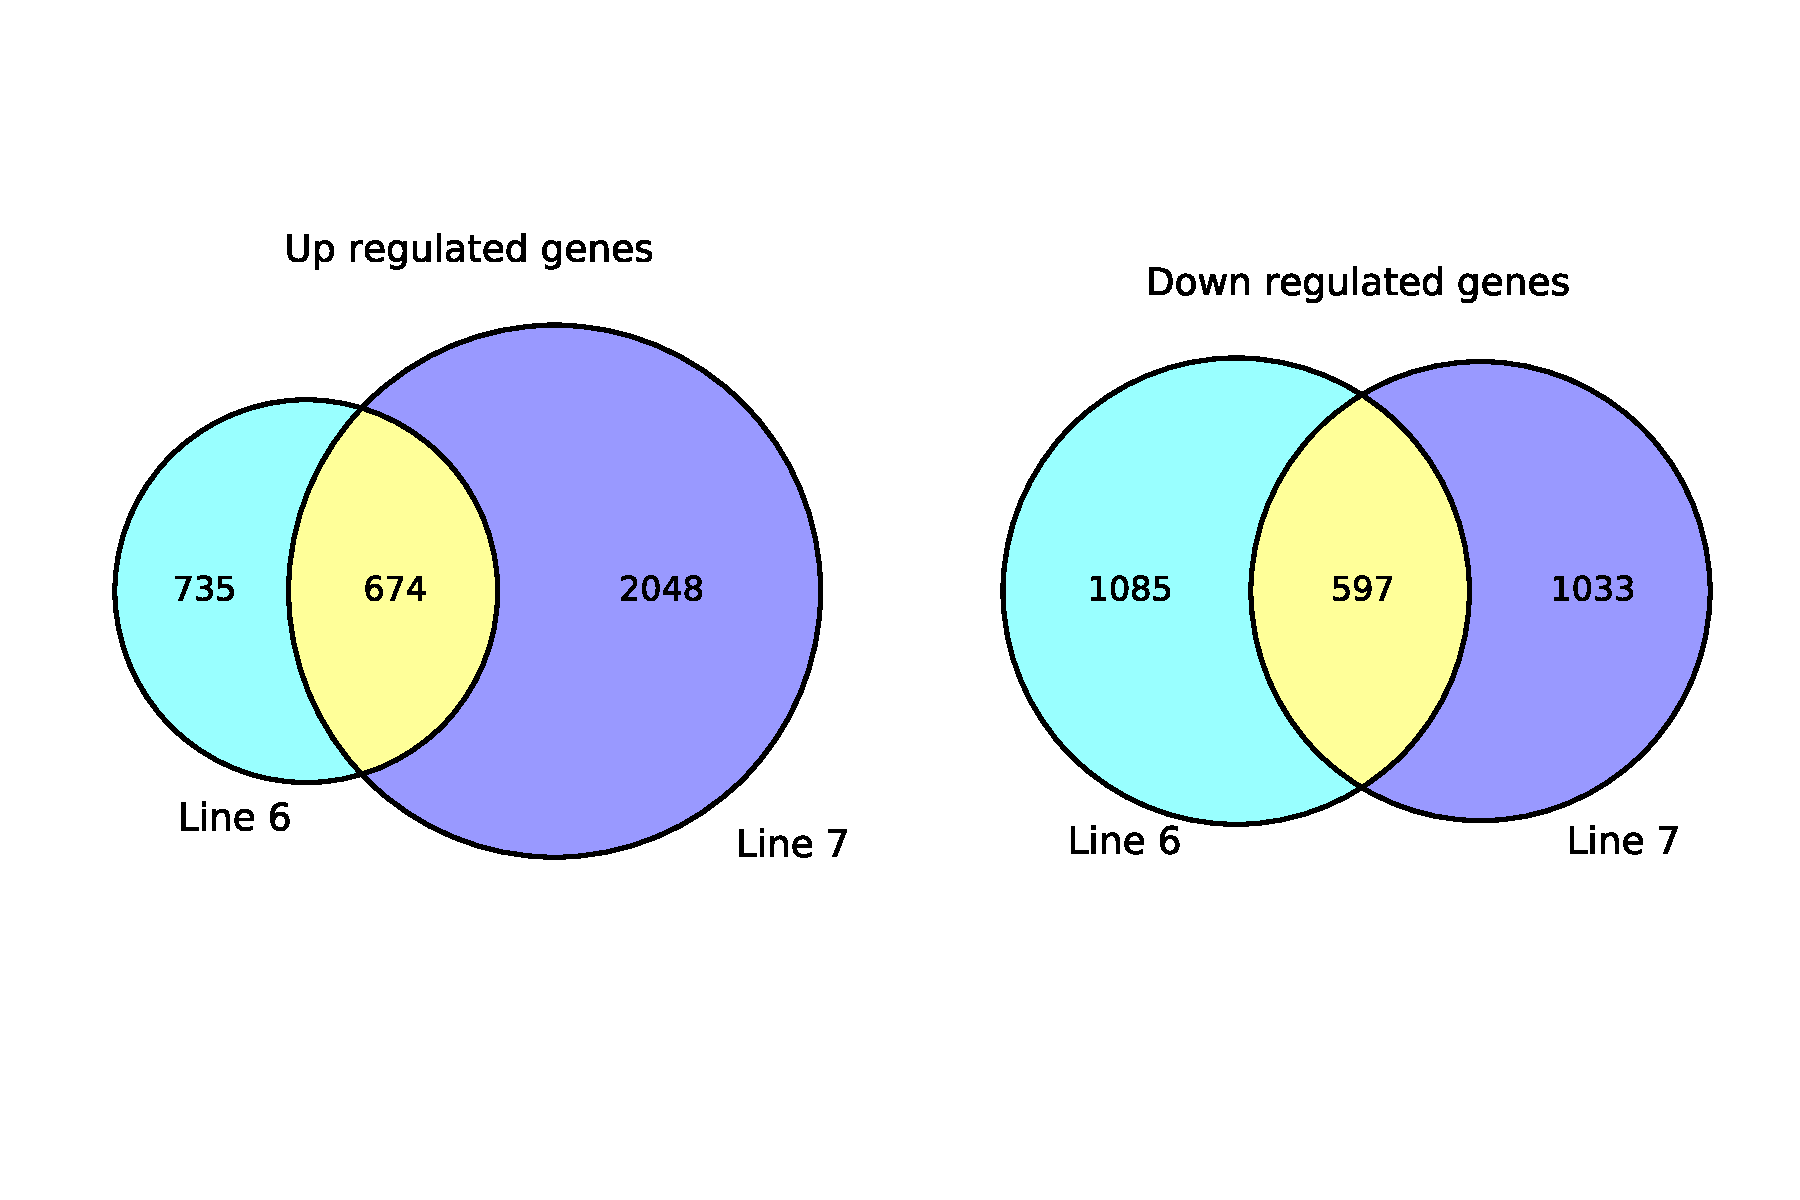
\includegraphics[width=6in]{degenes_venn.pdf}
    \end{center}
    \caption{
        \textbf{Differential-expressed genes in response to MDV
        infection.}
        More genes are differentially expressed between control
        and infected chickens from line 7 than line 6.
    }
    \label{degenes_venn_diagram}
\end{figure}

Interestingly, some genes that were differentially expressed in
both lines were regulated in the opposite direction
(Table~\ref{tab:opposite}).  Among genes downregulated in the
resistant line but upregulated in the susceptible line were {\em
LL} (lung lectin) and {\em SFTPA1}, which encode a
calcium-dependent C-type lectin and a lung surfactant protein
respectively.  Both molecules are important in innate
immunity~\cite{hogenkamp2008chicken,kingma2006defense}.  {\em
LIMS1} is involved in cell differentiation and proliferation and
{\em PPARG} is a suppressor of the {\em NF$\kappa$B}-mediated
proinflamatory response.  On the other hand, nearly all genes
upregulated in the resistant line but downregulated in the
susceptible line are involved in cell survival such as mRNAs
splicing, cell growth, and protein synthesis, except CD7 whose
function is involved in T cell-B cell interaction.  This
difference suggests that even at this stage of infection in the
resistant line, the lytic phase could be repressed. Therefore,
only genes involved in cell division are upregulated possibly to
repair the initial damage due to infection in the resistant line.
In comparison, the lytic phase in the susceptible line may still
continue and as a result, genes involved in immune responses are
still upregulated.

\clearpage\pagestyle{lscape}
\begin{landscape}
\begin{table}
\caption{
\textbf{Genes regulated in opposite directions in response to MDV
infection}
}
\begin{center}
    \begin{tabular}{cccc}
        \hline
        Gene & Description & $log_{2}$FC & \\
         & & Resistant & Susceptible\\
        \hline
        LL & Lung lectin & -3.36 & 8.71 \\
        GIF & Gastric intrinsic factor & -2.15 & 3.11 \\
        C14ORF1 & Chromosome 14 open reading frame 1 & -3.11 & 2.71 \\
        SFTPA1 & Surfactant protein A1 & -4.84 & 3.73 \\
        SCAF8 & SR-related CTD-associated factor 8 & -8.71 & 8.25 \\
        PPARG & Peroxisome proliferator-activated receptor frame 1 & -6.99 & 2.06 \\
        \hline
        NDUFA4 & NADH dehydrogenase (ubiquinone) 1 alpha subcomplex, 4 & 1.66 & -1.03 \\
        RAD17 & RAD17 homolog ({\em S. pombe})& 1.45 & -1.80 \\
        RPL39 & Ribosomal protein L39 & 3.34 & -1.63 \\
        ATP8A2 & ATPase, aminophospholipid transporter, class I, type 8A, member 2 & 7.66 & -7.80 \\
        NDUFB3 & NADH dehydrogenase (ubiquinone) 1 beta & 1.03 & -1.34 \\
        PSMG3 & Proteosome assembly chaperone 3 & 1.52 & -1.26 \\
        MED9 & Mediator complex subunit 9 & 8.23 & -3.15 \\
        PNISR & PNN-interacting serine/arginine-rich protein & 5.58 & -1.81 \\
        S1PR1 & Sphingosine-1-phosphatase receptor 1 & 1.31 & -6.96 \\
        CD7 & CD7 molecule & 2.88 & -1.38 \\
        LOC100858785 & Unknown & 1.26 & -1.75 \\
        THOC7 & THO complex 7 homolog (Drosophila) & 7.01 & -6.90 \\
        DNAJA2 & DnaJ (Hsp40) homolog, subfamily A, member 1 & 2.34 & -6.02 \\
        \hline
    \end{tabular}
    \begin{flushleft}
        (-) down-regulated, (+) up-regulated
    \end{flushleft}
    \label{tab:opposite}
\end{center}
\end{table}
\end{landscape}
\pagestyle{plain}

In addition, type I interferon ({\em IFN-$\gamma$} and {\em
IFN-$\beta$}) as well as {\em INF-$\alpha$3} were found to be
highly upregulated in infected chickens in both lines
(Table~\ref{tab:cytokines}).
% @Jerry: not exactly
However, expression of genes encoding their corresponding
receptors were not different in the resistant line, but
upregulated in the susceptible line.  This could also reflect the
ongoing immune response in the susceptible line.

\begin{table}[!ht]
\caption{
\textbf{Cytokine-related gene expression in response to MDV infection}}
\begin{center}
    \begin{tabular}{c>{\centering}m{7cm}cccc}
        \hline
        & & $log_{2}$FC & \\
        Symbol & Description & Resistant & Susceptible \\
        \hline
        IL2RG & Interleukin 2 receptor, $\gamma$ & -- & 0.55 \\
        IL6 & Interleukin 6 (interferon, $\beta$ 2) & -- & 5.11 \\
        IL6ST & Interleukin 6 signal transducer (gp130, oncostatin M receptor) & -- & 1.36 \\
        IL8L1 & Interleukin 8-like 1 & 1.90 & -- \\
        IL15 & Interleukin 15 & -- & 1.06 \\
        IL18 & Interleukin 18 (interferon-$\gamma$ inducing factor) & 1.92 & 4.07 \\
        IL18R1 & Interleukin 18 receptor 1 & 1.94 & 1.64 \\
        IFNG & Interferon-$\gamma$ & 5.14 & 4.90 \\
        IFNB & Interferon-$\beta$ & 4.83 & 5.64 \\
        IFNA3 & Interferon-$\alpha$ 3 & 4.09 & 5.48 \\
        IFNGR1 & Interferon-$\gamma$ receptor 1 & -- & 2.04 \\
        IFNGR2 & Interferon-$\gamma$ receptor 2& -- & 0.50 \\
        IFNAR1 & Interferon-$\alpha$,$\beta$ receptor 1 & -- & 1.46 \\
        IFNAR2 & Interferon-$\alpha$,$\beta$ receptor 2 & -- & 0.58 \\
        \hline
    \end{tabular}
    \begin{flushleft}
    \end{flushleft}
    \label{tab:cytokines}
\end{center}
\end{table}
\subsection{Functional analysis of differential-expressed genes
indicates inactive adaptive immune responses in the resistant
line}

To determine pathways that were perturbed during the infection,
data were analyzed by GOSeq, which accounts for gene length bias
unique to the RNA-Seq data~\cite{young2010method}.  Significantly
perturbed pathways (FDR $< 0.1$) from both lines that involved in
immune response include the TLR signaling pathway,
cytokine-cytokine receptor interaction, intestinal immune network
for IgA production, and cell Jak-STAT signaling pathway
(Figure~\ref{line67_kegg}). Some other pathways important in
response to viral infection and only significantly enriched in
the susceptible line include phagosome, apoptosis, RIG-I-like
receptor signaling pathway, NOD-like receptor signaling pathway,
and lysosome. For the phagosome pathway, a pathway that includes
genes important for stimulation of the adaptive immune response,
although MHC class I ({\em BF1}) was differentially expressed in
both lines, other genes involved in expressing newly synthesized
MHC class I were only upregulated in the susceptible line
suggesting that new MHC I molecules were actively produced.
Furthermore, Gene Ontology analysis of biological processes
(GO:BP) (data not shown) shows that categories involved in both
adaptive and innate immune responses were enriched in the
susceptible line.  On the other hand, only categories involved in
innate immune responses were enriched in the resistant line.  In
addition, enrichment of the apoptosis pathway in the susceptible
line suggests that the programmed cell death could be induced by
the CTL response to eliminate ongoing viral infection.

\begin{figure}[!ht]
    \begin{center}
        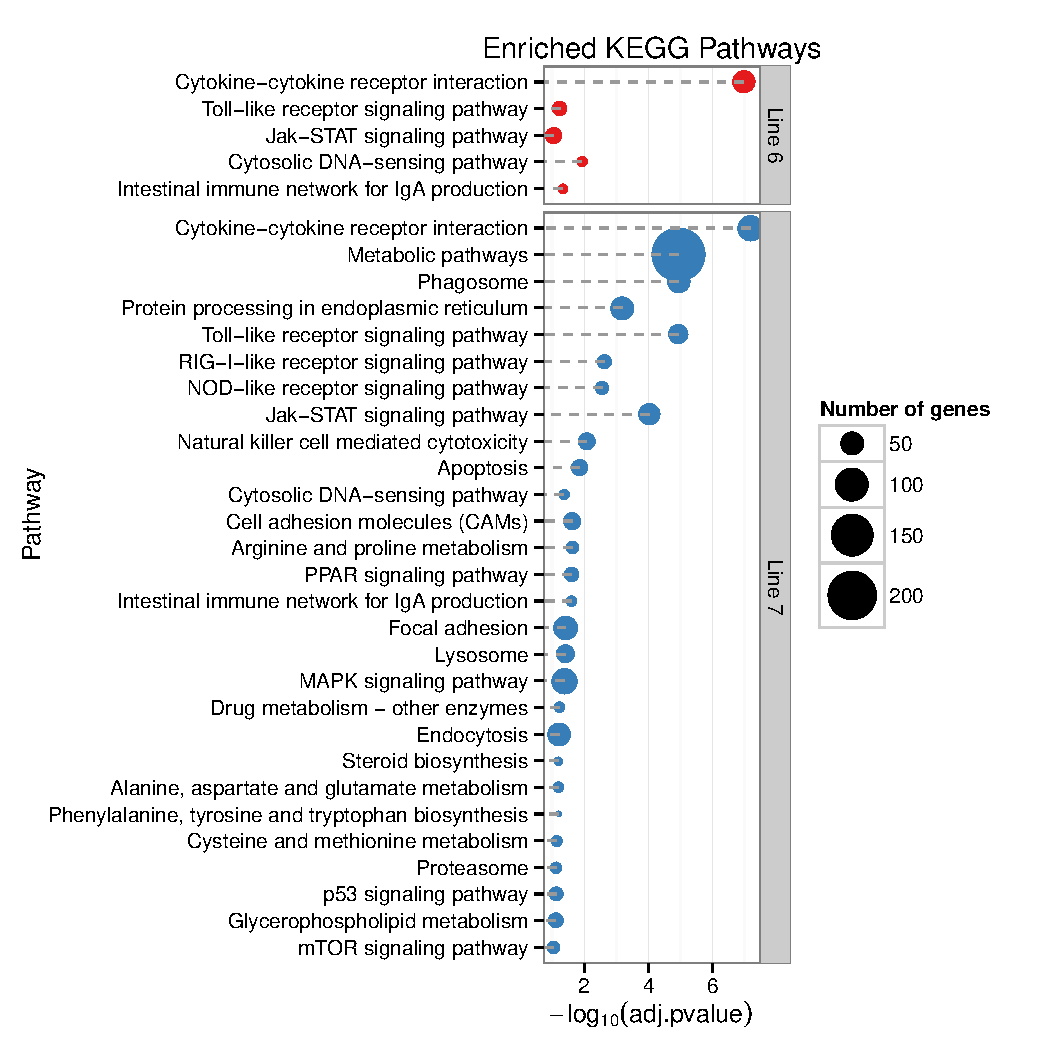
\includegraphics[width=7in]{line67_KEGG_cleveland.pdf}
    \end{center}
    \caption{
        \textbf{Enriched KEGG pathways.}
        Significantly enriched KEGG pathways from differentially
        expressed genes from lines 6 and 7 by GOSeq (FDR<0.1).
    }
    \label{line67_kegg}
\end{figure}

% \clearpage\pagestyle{lscape}
% \begin{landscape}
% \begin{figure}[!ht]
%     \begin{center}
%         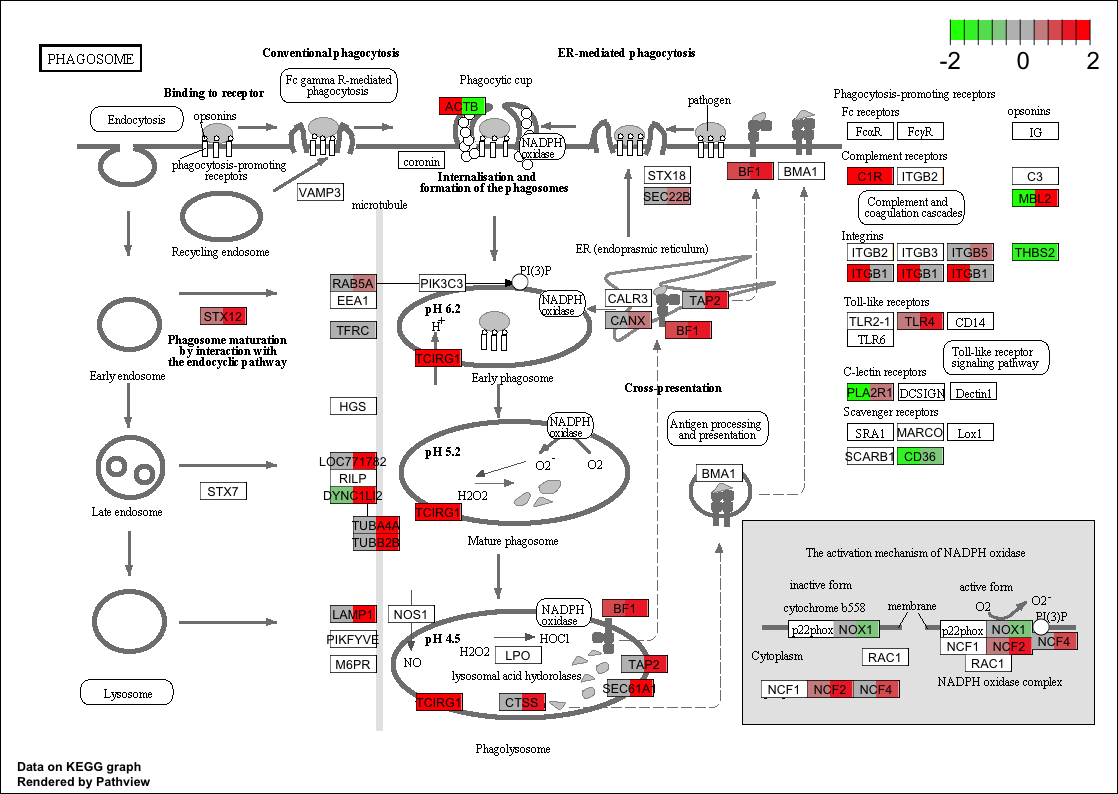
\includegraphics[width=8in]{gga04145_degenes_multi.png}
%     \end{center}
%     \caption{
%         \textbf{Phagosome pathway.}
%     }
%     \label{kegg_phagosome}
% \end{figure}
% \end{landscape}
% \pagestyle{plain}

At this stage of infection, our results suggest that lytic infection
of MDV stimulates both innate and adaptive immune responses, which
leads to activation of T cells in the susceptible line.  Only
activated T cells are believed to be infected by MDV, therefore, the
lytic phase could facilitate the spread of the viruse by enhancing
expansion of activated T cells.  Due to the cell-associate nature of
MDV, the viruses transfer to T cells via cell-to-cell contact between
B cells and T cells during antigen presentation or B cell activation
by T helper cells.  Therefore, it is beneficial for the host to
restrain such contact.  However, it is not clear how chickens in the
resistant line control the lytic infection of MDV.  Two mechanisms
have been speculated to contribute to MD resistance.  First innate
immune responses could be highly effective and could activate strong
adaptive immune responses that rapidly control viral replication and
force the viruses to enter into the latent phase.  Second, the innate
immune responses itself could be highly effective in limiting viral
replication~\cite{smith2011systems}.


\subsection{Genes with differential exon usage (DEU) in response
to MDV infection can be divided into four groups based on their
patterns of expression}

The immune system is isoform-rich and many genes express different
isoforms with distinctive functions in response to stimuli such as
stress, chemicals and infection.  Changes in expression of splice
forms of immune related genes have been reported to be associated with
increased susceptibility to and poor prognosis, of
diseases~\cite{lynch2004consequences}.  Studying differential isoform
expression could therefore shed light into inherent differences
between lines that confer resistance or susceptibility to MD.

In the past decades, microarray technology has been used to study gene
and isoform expression in many studies, but its sensitivity for
detection of structurally similar isoforms is low, and known or
predicted annotations are required to design
probes~\cite{kane2000assessment}.  Although the RNA-Seq method can
provide a reliable estimate of exon expression compared to
microarrays~\cite{pan2008deep} and is not constrained to the same
limitations, studying isoform expressions using RNA-Seq is still not
straightforward because of the short read lengths.  Reads from current
Illumina technology are generally not long enough to span across all
exons in an isoform.  In most cases, only exons in close proximity are
covered by the same read, which makes it difficult to accurately
predict a full structure of the isoform.  In addition, some genes are
fused due to overlapping untranslated regions (UTRs), which can also
result in erroneous predicted isoform structures.

Due to those issues, it is not feasible to accurately estimate
expression of isoforms, especially when gene annotation is constructed
from {\em de novo} assembly~\cite{trapnell2013differential}.  To avoid
these issues, we chose to study exon expression instead of isoform
expression.  Using MISO with the exon-centric method, only reads
spanning across a few exons are used and only exons involved in a
splicing event are examined.  The expression of exon inclusion is
calculated as Percent Spliced In (Psi or $\Psi$), which can be used to
infer the portion of transcripts that include the exon in each
sample~\cite{Katz:2010iv}.  In this study, we investigated the three
most common alternative splicing events in vertebrates, which are
skipped exons (SE), an alternative $3\prime$ (A3SS) and $5\prime$
(A5SS) splice site.  Lists of DEU genes from the resistant line that
show difference in $\Psi$ greater than 0.20 when compared to the
susceptible line in infected chickens are shown in
Tables~\ref{tab:line67i_diff_line67u_one},~\ref{tab:line67i_diff_line67u_two}
and~\ref{tab:line67i_diff_line67u_three}.  Genes can be categorized
roughly into four groups based on the pattern of $\Psi$ across control
and infected birds in both lines.

Group I (Table~\ref{tab:line67i_diff_line67u_one}) includes genes
with $\Psi$s that were up- or down-regulated in infected chickens
in the resistant line only.  This group includes {\em BCL11B}
(B-cell CLL/lymphoma 11B zinc finger proteins), a B-cell lymphoma
associated C2H2-type zinc finger protein encoding gene, which
functions as a tumor-suppressor for T-cell lymphoma in human.
According to homologous alignments on the UCSC genome browser, a
splice form with the skipped exon is similar to mouse {\em BCL11B
isoform b}.  The skipped exon was expressed 30\% in the infected
chickens from the resistant line; whereas it was rarely expressed
(4-7\%) in the control resistant line and both groups in the
susceptible line.  The skipped exon was not found to encode any
known protein domain, however, it is in the middle of two
adjacent C2H2-type finger protein domains. {\em GEMIN6} plays a
role in the assembly of spliceosomal snRNP in cytoplasm.  {\em
SRSF6} (SR splicing factor 6) encodes a nuclear protein that
belongs to the splicing factor protein family.

In group II (Table~\ref{tab:line67i_diff_line67u_two}), $\Psi$
values were relatively stable in control and infected chickens
within line, but not between lines.  Genes that could play an
important role in immune responses are {\em RAC3}, {\em HCK}, and
{\em ITGB2}.  {\em RAC3} (Ras-related C3 botulinum toxin This
gene encodes small GTPases, belonging to the Ras family, that
regulate a wide variety of cellular events including cell growth,
cytoskeletal reorganization, and the activation of protein
kinases.  The role of small GTPases in immune responses is
discussed further below.  {\em HCK} transmits signals from cell
surface receptors such as {\em FCGR1A, FCGR2A, IL2, IL6, IL18},
and integrins ({\em ITGB1, ITGB2}).  {\em ITGB2} (CD18) encodes
subunit $\beta_{2}$ integrin of {\em LFA-1} and {\em CR3}
receptors.  {\em LFA-1} plays an important role in adhesion of
lymphocytes with other cells.  {\em CR3} binds to a vast array of
ligands and molecules including complement C3bi, microbial
proteins, ICAM-1 and -2, ECM proteins, and coagulation proteins.
It plays a significant role in neutrophil and monocyte activation
including phagocytosis, adhesion and migration.  The role of {\em
ITGB2} in immune responses is discussed further in the next
section. {\em DYNLL2, SEPT11} and {\em PFN2} are also involved in
cell rearrangement and cytokinesis.  In particular, {\em DYNLL2}
is a dynein protein that have been demonstrated to regulate T
cell activation by driving T cell receptor microclusters
(TCR-MCs) toward the center of an immune
synapse~\cite{hashimoto2011dynein}.

Group III (Table~\ref{tab:line67i_diff_line67u_three}) includes
genes that exhibit differential isoform expression only in
response to the infection in susceptible line.  A number of genes
in this group encode proteins that are parts of spliceosome: {\em
SRSF3}, {\em HNRNPDL}, {\em SFSWAP}, {\em THOC1}, {\em RNPC3} and
{\em SRSF5}.  {\em PODXL} encodes PODX-like proteins that
function in an integrin-dependent manner as both pro-adhesive and
anti-adhesive molecules.  This protein is involved in
cell-to-cell contact, cell trafficking, and cancer
progression~\cite{nielsen2009role,somasiri2004overexpression}.

The last group (Group IV,
Table~\ref{tab:line67i_diff_line67u_three}) only has three genes:
{\em GOSR1}, {\em SRSF6} and {\em ENSGAL00000026498}.  The $\Psi$
value differences of these genes were greater than 0.20 the
cutoff between control and infected chickens in the resistant and
susceptible lines and were significantly different between
infected chickens in the resistant and susceptible lines. {\em
GOSR2} encodes a trafficking membrane protein important for
transporting proteins from the {\em cis-} to the {\em
trans-}golgi network and {\em SRSF6} (serine/arginine-rich
splicing factor 6) encodes a protein involved in mRNA splicing.

\clearpage\pagestyle{lscape}
\begin{landscape}
\begin{table}[!ht]
\caption{
\textbf{DEU between the resistant line and the susceptible line
in infected birds, group I}}
\begin{center}
\begin{tabular}{cccccccc}
\hline
& & & Resistant ($\Psi$) & & Susceptible ($\Psi$) & \\
Type & Ensembl & Symbol  & Un & Inf & Un & Inf \\
\hline
SE & ENSGALG00000011127 & BCL11B & 0.07 & \textbf{0.30} & 0.06 & 0.04 \\
SE & ENSGALG00000013137 & INO80C & 0.15 & \textbf{0.35} & 0.95 & 0.86 \\
A5SS & ENSGALG00000013821 & GEMIN6 & 0.84 & \textbf{0.61} & 0.81 & 0.85 \\
A5SS & ENSGALG00000009824 & C7H2ORF77 & 0.49 & \textbf{0.26} & 0.68 & 0.62 \\
A5SS & ENSGALG00000002144 & THRAP3 & 0.31 & \textbf{0.51} & 0.28 & 0.18 \\
A3SS & ENSGALG00000020987 & ZDHHC7 & 0.42 & \textbf{0.23} & 0.57 & 0.55 \\
A3SS & ENSGALG00000005685 & KSR1 & 0.77 & \textbf{0.44} & 0.72 & 0.65 \\
A3SS & ENSGALG00000027665 & SYNGR1 & 0.46 & \textbf{0.23} & 0.68 & 0.60 \\
A3SS & ENSG00000163875* & MEAF6 & 0.28 & \textbf{0.57} & 0.40 & 0.29 \\
\hline
\end{tabular}
\begin{flushleft}
    *Human homologs, Un=uninfected, Inf=infected, SE=skipped exon,
    A5SS=$5\prime$ splice site, A3SS=$3\prime$ splice site.  Bold face
    indicates that there is a SNP between the lines 6 and 7
    within an alternative exon.
\end{flushleft}
\label{tab:line67i_diff_line67u_one}
\end{center}
\end{table}

\begin{table}[!ht]
\caption{
\textbf{DEU between the resistant line and the susceptible line
in infected birds, group II}
}
\begin{center}
\begin{tabular}{cccccccc}
\hline
& & & Resistant ($\Psi$) & & Susceptible ($\Psi$) & \\
Type & Ensembl & Symbol  & Un & Inf & Un & Inf \\
\hline
SE & ENSGALG00000005522 & DYNLL2 & \textbf{0.01} & \textbf{0.02} & 0.20 & 0.25 \\
SE & ENSGALG00000004971 & URM1 & \textbf{0.07} & \textbf{0.03} & 0.18 & 0.23 \\
SE & ENSGALG00000015709 & TACC3 & \textbf{0.87} & \textbf{0.93} & 0.77 & 0.72 \\
SE & ENSGALG00000014642 & LOC374195 & \textbf{0.60} & \textbf{0.57} & 0.70 & 0.80 \\
SE & ENSGALG00000011682 & CNOT4 & \textbf{0.57} & \textbf{0.62} & 0.40 & 0.41 \\
SE & ENSGALG00000007511 & ITGB2 & \textbf{0.17} & \textbf{0.22} & 0.02 & 0.01 \\
SE & ENSGALG00000006522 & HCK & \textbf{0.47} & \textbf{0.59} & 0.99 & 0.97 \\
SE & ENSGALG00000000904 & C11H16ORF57 & \textbf{0.92} & \textbf{0.98} & 0.84 & 0.78 \\
A5SS & ENSGALG00000010836 & AHR & \textbf{0.97} & \textbf{0.99} & 0.63 & 0.59 \\
A5SS & ENSGALG00000011488 & CMTM7 & \textbf{0.55} & \textbf{0.67} & 0.37 & 0.41 \\
A3SS & ENSGALG00000008939 & FUBP1 & \textbf{0.42} & \textbf{0.26} & 0.59 & 0.54 \\
A3SS & ENSGALG00000008507 & THOC2 & \textbf{0.52} & \textbf{0.53} & 0.69 & 0.78 \\
A3SS & ENSGALG00000002859 & RAC3 & \textbf{0.69} & \textbf{0.84} & 0.67 & 0.61 \\
A3SS & ENSGALG00000012050 & TNRC6B & \textbf{0.57} & \textbf{0.39} & 0.94 & 0.93 \\
A3SS & ENSGALG00000010410 & PFN2 & \textbf{0.71} & \textbf{0.78} & 0.53 & 0.50 \\
A3SS & ENSGALG00000027908 & LOC422528 & \textbf{0.28} & \textbf{0.39} & 0.13 & 0.09 \\
A3SS & ENSGALG00000011476 & SEPT11 & \textbf{0.78} & \textbf{0.86} & 0.60 & 0.58 \\
\hline
\end{tabular}
\begin{flushleft}
    *Human homologs, Un=uninfected, Inf=infected, SE=skipped exon,
    A5SS=$5\prime$ splice site, A3SS=$3\prime$ splice site.  Bold face
    indicates that there is a SNP between the lines 6 and 7
    within an alternative exon.
\end{flushleft}
\label{tab:line67i_diff_line67u_two}
\end{center}
\end{table}

\begin{table}[!ht]
\caption{
\textbf{DEU between the resistant line and the susceptible line
in infected birds, group III and IV}}
\begin{center}
\begin{tabular}{cccp{2cm}cccc}
\hline
& & & Resistant ($\Psi$) & & Susceptible ($\Psi$) & \\
Type & Ensembl & Symbol  & Un & Inf & Un & Inf \\
\hline
SE & ENSGALG00000003861 & HERC4 & 0.31 & 0.37 & 0.45 & \textbf{0.06} \\
SE & ENSGALG00000009029 & TSPAN12 & 0.08 & 0.15 & 0.20 & \textbf{0.47} \\
SE & ENSGALG00000009520 & MARCH1 & 0.42 & 0.54 & 0.66 & \textbf{0.34} \\
SE & ENSGALG00000008320 & EDEM1 & 0.95 & 0.99 & 0.90 & \textbf{0.72} \\
SE & ENSGALG00000000533 & SRSF3 & 0.36 & 0.38 & 0.30 & \textbf{0.16} \\
SE & ENSGALG00000023199 & HNRPDL & 0.39 & 0.40 & 0.30 & \textbf{0.18} \\
SE & ENSGALG00000006157 & DDX26B & 0.67 & 0.60 & 0.57 & \textbf{0.84} \\
SE & ENSGALG00000001745 & PSTPIP2 & 0.07 & 0.05 & 0.11 & \textbf{0.26} \\
SE & ENSG00000175029* & CTBP2 & 0.38 & 0.38 & 0.23 & \textbf{0.12} \\
A5SS & ENSGALG00000008038 & SF3B1 & 0.41 & 0.57 & 0.55 & \textbf{0.31} \\
A5SS & ENSGALG00000002487 & SFSWAP & 0.58 & 0.73 & 0.55 &
\textbf{0.41} \\
A3SS & ENSGALG00000005162 & RNPC3 & 0.55 & 0.36 & 0.42 & \textbf{0.67} \\
A3SS & ENSGALG00000000720 & LOC419563 & 0.88 & 0.94 & 0.85 &
\textbf{0.70} \\
A3SS & ENSGALG00000009421 & SRSF5 & 0.55 & 0.72 & 0.54 & \textbf{0.39} \\
A3SS & ENSGALG00000014915 & THOC1 & 0.33 & 0.48 & 0.33 & \textbf{0.23} \\
A3SS & ENSGALG00000000189 & YTHDC2 & 0.44 & 0.59 & 0.42 &
\textbf{0.32} \\
\hline
SE & ENSGALG00000001107 & GOSR2 & 0.73 & \textbf{0.92} & 0.38 &
\textbf{0.59} \\
SE & ENSG00000124193* & SRSF6 & 0.43 & \textbf{0.71} & 0.54 &
\textbf{0.34} \\
A3SS & ENSGALG00000026498 & Unknown & 0.12 & \textbf{0.70} & 0.10 &
\textbf{0.34} \\
\hline
\end{tabular}
\begin{flushleft}
    *Human homologs, Un=uninfected, Inf=infected, SE=skipped exon,
    A5SS=$5\prime$ splice site, A3SS=$3\prime$ splice site.  Bold face
    indicates that there is a SNP between the lines 6 and 7
    within an alternative exon.
\end{flushleft}
\label{tab:line67i_diff_line67u_three}
\end{center}
\end{table}
\end{landscape}
\pagestyle{plain}

\subsection{Roles of {\em LFA-1} and actin cytoskeleton in T
cells activation}

By grouping genes based on patterns of $\Psi$s, we found that many
genes in group II: {\em ITGB2, PFN2, DYNLL2, SEPT11}, and {\em
RAC3}, are involved in cytokinesis or cell synapse, which are
important for T cell activation.  As described above, {\em ITGB2}
encodes the $\beta$-subunit of integrins including LFA-1, which is
exclusively expressed in lymphocytes and plays a major role in
lymphoproliferation, antigen presentation, T cell activation, and
cytotoxicity.  Integrins are special kind of receptors that transmit
signals bidirectionally across the cell membrane.  They are
heterodimeric composed of an $\alpha$ (large) and a $\beta$ (small)
subunit~\cite{wang2010immunopathologies}.  The $\beta_{2}$ (CD18)
subunit encoded by {\em ITGB2} is expressed on lymphocytes and antigen
presenting cells (APCs) as a component of {\em LFA-1} and {\em CR3}
receptors.  LFA-1 binds to its ligand ICAM-1 to help form a synapse
that brings APCs and T cells together to initiate antigen presentation
leading to T cell activation~\cite{dustin2000immunological}.

Absence of LFA-1 leads to impaired functions of lymphocytes in
proliferation and tumor
rejection~\cite{scharffetter1998spontaneous,schmits1996lfa}.
Mutations in the {\em ITGB2} gene have been associated with type 1
leukocyte adhesion deficiency (LAD-1), an autosomal-recessive
inherited disease found in a few families.  The disease is
characterized by impairment of lymphocytes in adherent-dependent
functions, lack of accumulation to the site of infection and recurrent
bacterial and fungal infection~\cite{springer1987lymphocyte}.  In
addition, the response of lymphocytes to mitogens is decreased in
patients with LAD~\cite{springer1987lymphocyte}.  The decrease in
responsiveness to mitogens has been shown to correlate with resistance
to MD by Lee and Bacon~\cite{lee1983ontogeny}, who illustrated that
resistant birds (MD resistant lines 6 and N) were less responsive to
phytohemagglutinin (PHA) than MD susceptible birds (line 7 and P).

The actin cytoskeleton is very important in T cell activation because
it enhances the activity of LFA-1 by increasing its avidity and
recruiting signaling molecules necessary for downstream
signaling~\cite{dustin2000immunological, van2000avidity}.
Cytoskeleton proteins binding to cytoplasmic domain of LFA-1 are
thought to play an important role in driving LFA-1 to aggregate
on the cell surface, resulting in increased avidity.  Aggregation
of LFA-1 has been demonstrated to be essential for lymphocytes to
bind to the ligand~\cite{van1994extracellular}.  Interestingly,
{\em RAC3} and {\em PFN2}, which are involved in the actin
cytoskeleton pathway (Figure~\ref{kegg_actin}), also expressed
different ratios of alternative splice forms between lines .
These gene products are also found in three other pathways
that are involved in immune responses (Table~\ref{tab:integrin}).  It
could be speculated that pre-mRNA splicing of these genes is
co-regulated by splicing regulators or some genetic factors.

\begin{figure}[!ht]
    \begin{center}
        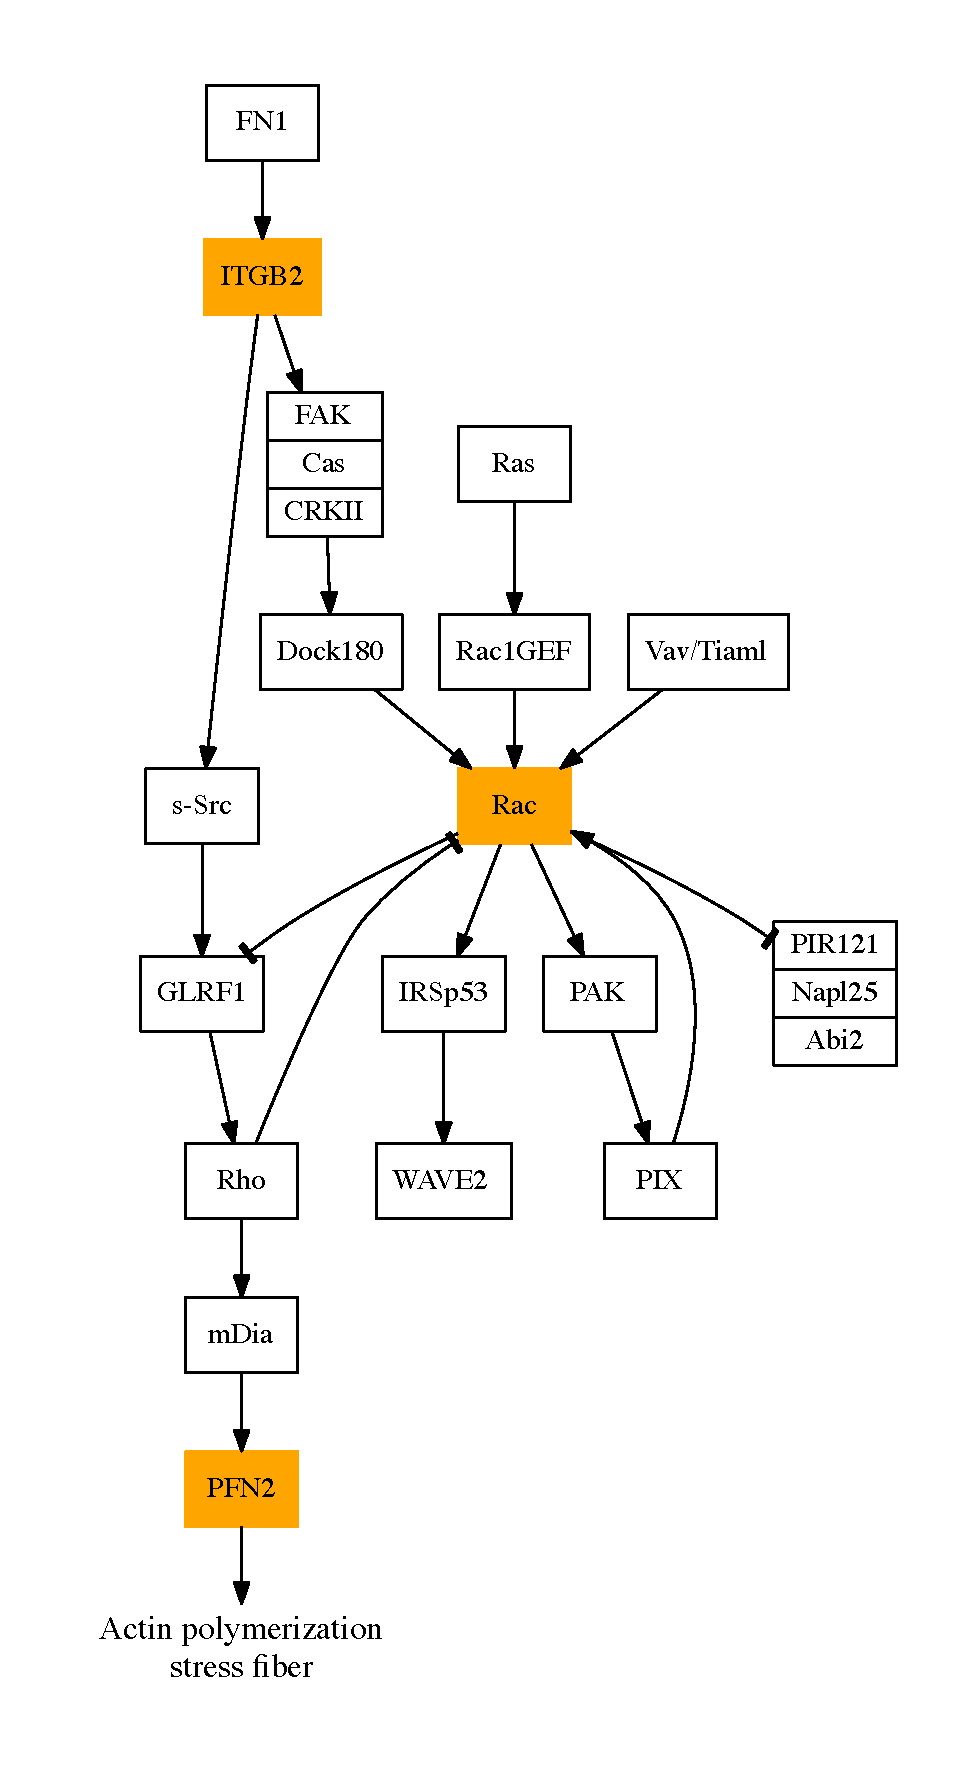
\includegraphics[width=4in]{hsa04810.pdf}
    \end{center}
    \caption{
        \textbf{Human regulation of actin cytosekeleton pathway.}
        An exon of {\em ITGB2, RAC} and {\em PFN2} is not
        differentially expressed between the control and the
        infected groups, but between resistant and susceptible
        chickens. These three genes indirectly interact with one
        another in the pathway.  Only genes that interact with
        these genes are shown in this figure.
    }
    \label{kegg_actin}
\end{figure}

\begin{table}[!ht]
\caption{
\textbf{Pathways containing {\em RAC3, ITGB2} and {\em PFN2}}}
\begin{center}
\begin{tabular}{ccc}
\hline
Pathway ID &  Description & Gene \\
\hline
hsa04810 & Regulation of actin cytoskeleton & {\em RAC3, ITGB2, PFN2} \\
hsa04015 & RAP1 signaling pathway & {\em RAC3, ITGB2, PFN2} \\
hsa04650 & Natural killer cells cytotoxicity & {\em RAC3, ITGB2} \\
hsa05416 & Viral myocarditis & {\em RAC3, ITGB2} \\
\hline
\end{tabular}
\begin{flushleft}
\end{flushleft}
\label{tab:integrin}
\end{center}
\end{table}

\subsection{Prediction of functional domains of splice forms of
genes in the actin cytoskeleton pathway}

To predict the function of the alternative splice forms of genes in
the actin cytoskeleton pathway, transcript sequences were translated
to protein sequences by ESTscan~\cite{iseli1999estscan}.  Protein
sequences were then searched for annotated protein domains using the
standalone version of InterPro Scan~\cite{quevillon2005interproscan}.
Besides {\em ITGB2}, other genes have alternative exons located in
coding regions that could potentially affect functional protein
domains in some ways.  The exon with an alternative 3$\prime$ splice
site of {\em RAC3} encodes part of a protein domain identified as a
small GTPase of the Ras subfamily (ProSiteProfiles:PS5142 and
SMART:SM00173).  Rac3 is highly homologous to Rac1 and has been
reported to possess the ability to promote membrane ruffling,
transformation, activation of c-Jun transcriptional activity and
co-activation of NF$\kappa$B~\cite{werbajh2000rac}.  Activated Rac
also regulates production of superoxide in neutrophils and
macrophages.

The alternative exon of {\em PFN2} seems to disrupt the coding
sequence that encodes the profilin domain (Pfam:PF00235).  The
profilin domain is essential for almost all organisms and its
functions include regulating actin polymerization, controlling
complex networks of molecular interaction and transmitting signals
from small-GTPase pathways.  It also binds to Rac effector
molecules and a number of other ligands~\cite{witke2004role}.

Even though the exact mechanism is not known, lack of responsiveness
of T cells to stimuli appears to benefit resistant birds because in
these birds MDV can not induce T cells to proliferate and cause them
to undergo neoplastic transformation.  It has also been suggested that
the mechanism that controls both lymphocyte proliferation induced by
MDV and lymphocyte proliferation induced by the immune response is the
same~\cite{pazderka1975histocompatibility}.  Therefore, it may be
useful to consider a link between the deficiency of lymphocytes in the
resistant line to the alternative splice form of {\em ITGB2} that is
only expressed in the resistant line.  Although the exon included in
the alternative splice form is non-coding, it could serve important
functions in translation or posttranscriptional regulation.

\subsection{Prediction of {\em cis}-regulatory elements in
alternative splicing exons of genes in group II}

Among all groups, alternative splicing of genes in the group II is
most likely to be regulated by genetic factors because the ratios of
isoform expression in this group were relatively stable within line,
but were significantly different between lines.  Investigation of
nucleotide differences within exons of both lines could reveal a
possible role of SNPs in regulating alternative splicing in this
group.  We obtained a sequence of alternative exons from the
resistant line and used Human Splicing Finder (HSF) to determine
whether SNPs from the susceptible line could alter predicted ESEs or
ESSs.  Results from some genes involved in cytokinesis are discussed
in this section.  Exonic SNPs from the resistant and susceptible lines
are listed in Table~\ref{tab:deu_snps}.

\begin{table}[!ht]
\caption{
\textbf{SNP between resistant and susceptible lines found in an
exon of ITGB2, PFN2 and DYNNL2 (Group II)}}
\begin{center}
\begin{tabular}{ccccccc}
\hline
Gene &  Chromosome & Position & Reference & Resistant & Susceptible & Strand \\
\hline
ITGB2 & 7 & 7183696 & C & {\em T} & . & - \\
PFN2 & 9 & 23221934 & -  - & . & {\em AA} & + \\
DYNLL2 & 19 & 8694149 & G & . & {\em A} & - \\
\hline
\end{tabular}
\end{center}
\begin{flushleft}
\end{flushleft}
\label{tab:deu_snps}
\end{table}

For {\em ITGB2}, a SNP (T) at position 26 of the cDNA from the
resistant line, which corresponds to position 7,183,696 on
chromosome 7 is located in a predicted binding site for SC35,
which is an exon enhancer.  Although the exon is not expressed in
the susceptible line, we found that there is no polymorphisms
between lines according to SNP data from genome resequencing.
Therefore, this SNP may not account for exclusion of the exon in
the susceptible line (Figure~\ref{itgb2}).  Exon sequences of
{\em PFN2} from the lines 6 and 7 differ at position 23,221,934
on chromosome 9.  A small insertion of two AA nucleotides is
predicted to create a new binding site for Tra2-$\beta$ splicing
regulator, which serves as a stabilizer of an enhancer
complex~\cite{lopez1998alternative}
(Table~\ref{tab:spliceosome}).  From exon expression data, $\Psi$
of an exon with alternative splicing increases from 0.20-0.30 to
about 0.50 in the susceptible line.  Tra2 could possibly increase
inclusion of the exon with alternative 3$\prime$ splice site via
ESE-dependent 3$\prime$ splice site activation
(Figure~\ref{pfn2}).  Even though the linear distance between
Tra2-$\beta$ binding site and the alternative 3$\prime$ splice
site is greater than 1kb, Tra2 could possibly get close to the
3$\prime$ splice site in the secondary structure of the mRNA.

\clearpage\pagestyle{lscape}
\begin{landscape}
\begin{figure}[!ht]
    \begin{center}
        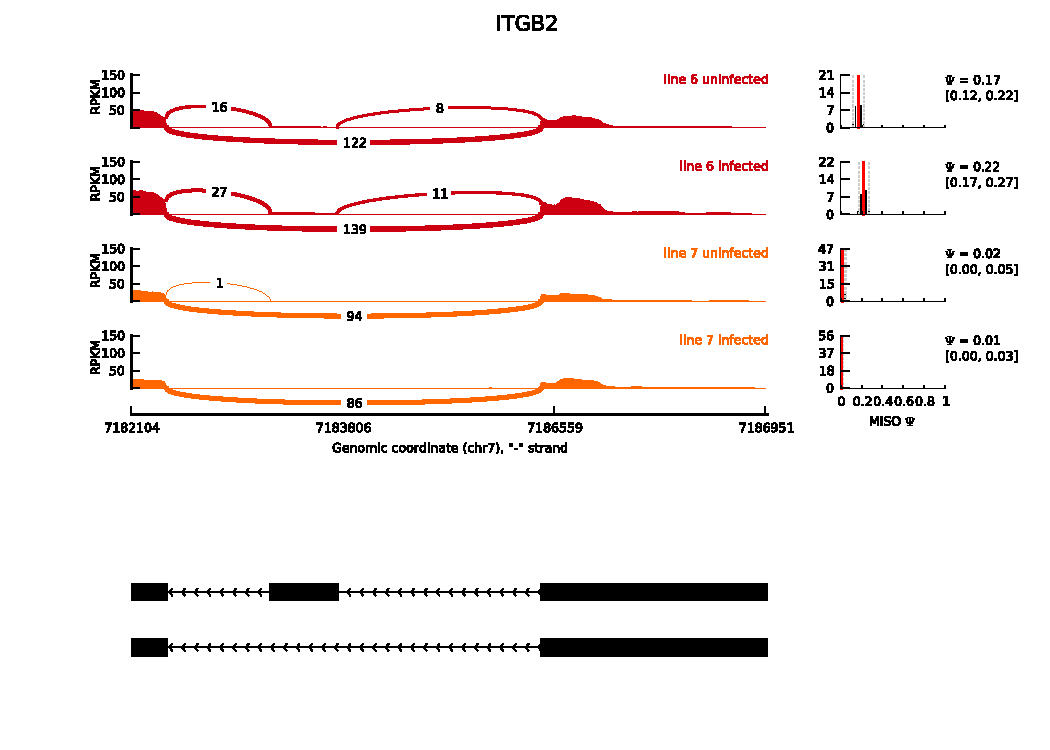
\includegraphics[width=7.5in]{itgb2_miso.pdf}
    \end{center}
    \caption{
        \textbf{ITGB2 exon expression.}
        The cassette exon is predicted to be skipped in line 7
        but expressed $\sim$20\% in line 6. The histogram depicts
        read coverage and the curve lines depict spliced reads. The
        distribution of $\Psi$ values are plotted on the right
        side with confidence intervals in the square brackets. At
        the bottom of the plot, black think horizontal lines
        depict exons and thin lines with arrow heads depict
        introns.
    }
    \label{itgb2}
\end{figure}
\begin{figure}[!ht]
    \begin{center}
        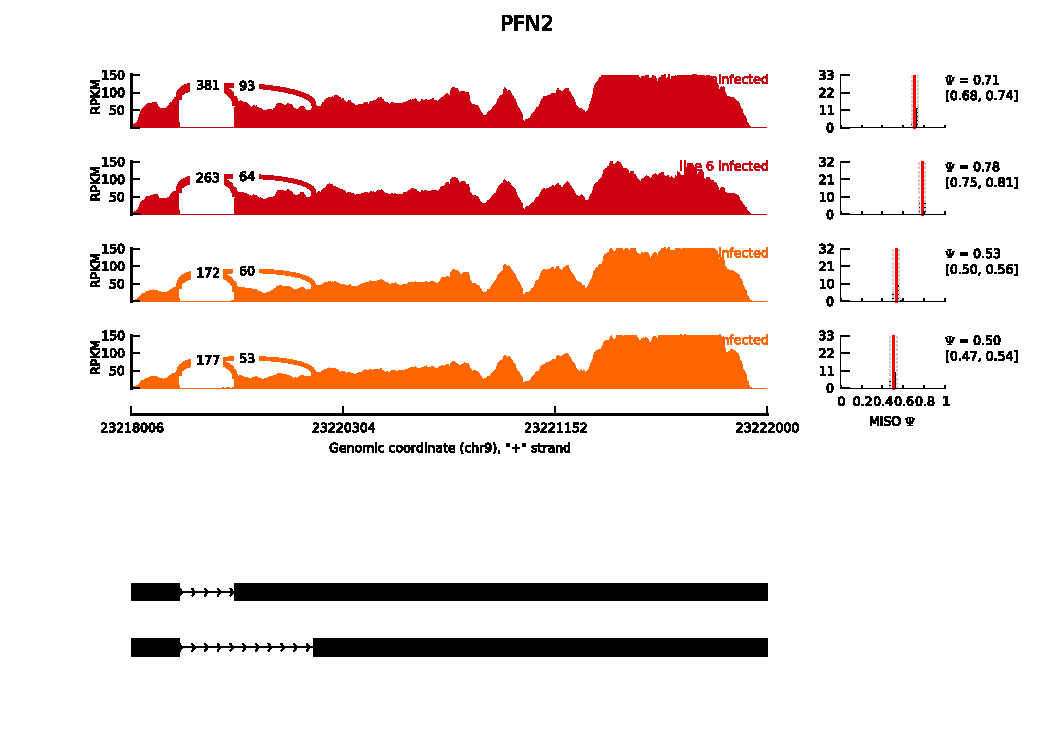
\includegraphics[width=7.5in]{pfn2_miso.pdf}
    \end{center}
    \caption{
        \textbf{PFN2 exon expression.}
        The long exon is predicted to be more expressed in line 6
        (control and infected group) than in line 7. The
        histogram depicts read coverage and the curve lines
        depict spliced reads. The distribution of $\Psi$ values
        are plotted on the right side with confidence intervals
        in the square brackets.  At the bottom of the plot, black
        think horizontal lines depict exons and thin lines with
        arrow heads depict introns.
    }
    \label{pfn2}
\end{figure}
\end{landscape}
\pagestyle{plain}


Replacement of an A with a G nucleotide in the skipped exon of
{\em DYNLL2} from line 6 is predicted to slightly alter the
binding site of several ESEs as well as to create a new binding
site for 9G8 (Table~\ref{tab:spliceosome}).  This exon is
upregulated in the susceptible line compared to the resistant
line, therefore, the presence of the new binding site for 9G8
exon enhancer helps support the expression results.  In addition,
the G nucleotide in this position matches the reference
nucleotide, therefore, we could expect this exon to be expressed
in other datasets.  According to EST tags on the UCSC genome
browser, the exon has been found and sequenced from chicken eyes
(15d post-hatched, EST sequence:DR424100).

\clearpage\pagestyle{lscape}
\begin{landscape}
\begin{table}[!ht]
\caption{
\textbf{Results from human splicing finder}}
\begin{center}
\begin{tabular}{lp{1cm}p{3cm}llll}
\hline
Gene &  cDNA Position & Linked SR protein & Type & Reference Motif & Mutant Motif & Variation \\
\hline
DYNLL2 & 2 & SF2/ASF (IgM-BRCA1) & ESE$^{1}$ & CTCCGGG (86.38) & CTCCGAG (72.69) & -15.85\% \\
& 2 & SF2/ASF, SF2/ASF (IgM-BRCA1) & ESE$^{1}$ & CTCCGGG (79.91) & CTCCGAG (72.69) & -9.03\% \\
& 4 & SF2/ASF (IgM-BRCA1) & ESE$^{1}$& CCGGGGT (73.00) & CCGAGGT (86.23) & 18.12\% \\
& 4 & SF2/ASF (IgM-BRCA1), SF2/ASF & ESE$^{1}$ & CCGGGGT (73.00) & CCGAGGT (82.94) & 13.61\% \\
& 6 & 9G8 & ESE$^{2}$ & & GAGGTG (60.67) & New site \\
& 6 & hnRNP A1 & ESS$^{4}$& & GAGGTG (74.05) & New site \\
\hline
PFN2 & 2068 & Tra2-$\beta$ & ESE$^{1}$ & AAAAT (81.02) & AAAAa & +16.19\% \\
& 2069 & Tra2-$\beta$ & ESE$^{1}$ & & AAAaa (94.14) & New site \\
& 2070 & Tra2-$\beta$ & ESE$^{1}$ & & AAAaaT (81.02) & New site \\
 & 2066 & & ESS$^{3}$ & & ACAAAAaa (38.13) & New site \\
 & 2067 & & ESS$^{3}$ & & CAAAAaaT (28.85) & New site \\
\hline
\end{tabular}
\begin{flushleft}
    $^{1}$ESE Finder matrices for SRp40, SC35, SF2/ASF and SRp55 proteins.
    $^{2}$ESE motifs from HSF.
    $^{3}$Predicted PESS Octamers from Zhang \& Chasin.
    $^{4}$hnRNP motif.
\end{flushleft}
\label{tab:spliceosome}
\end{center}
\end{table}
\end{landscape}
\pagestyle{plain}

There are too many SNPs in the exon of {\em SEPT11}, making it
unfeasible to predict which SNP might regulate the exon
expression.  Therefore, we do not discuss these two genes in this
section.  However, results from HSF analysis of these two genes
and other genes in this group are provided in the supplementary
materials.  Experimental validation of exonic SNPs provided by
this study could shed some light on underlying polymorphisms that
contribute to resistance to MD.

\section{Conclusion}

Custom gene models built from combination of gene models from {\em de
novo} assembly, reference-based assembly, and Ensembl have allowed us
to identify genes and isoforms that might play an important role in
resistance to MD.  Results from gene expression analysis indicated
that adaptive immune responses were more highly activated during lytic
infection in the susceptible line, than in the resistant line.
Because only activated T cells are thought to be infected by MDV, we
speculate that enhancement of adaptive immune responses could help
spread the viruses by recruiting and activating more T cells.  In
contrast, the delay or reduction of adaptive immune responses could
benefit the host by limiting infection of activated T cells.

To elucidate the molecular mechanism of MD resistance, we
investigated differential isoforms expression between lines  and
identified a number of genes that could be responsible for
difference in immune responses. Notably, this incudes several genes
involved in actin cytoskeleton structure and cytokinesis, which are
important for the functions of lymphocytes and immune cells but
have not been of great interest in the field of MD research.
Even though we mainly discuss the possible role of {\em ITGB2}
in MD resistance, other genes cannot be precluded and should be a
candidate for further investigation and experimental studies.
Moreover, the full mechanism of MD resistance is highly complex and
more data from different stages of infection as well as greater
sequencing depth will be required to identify all genes and
isoforms involved.  To enhance the study of unannotated gene and
isoform expression, our approach of constructing gene models from
RNA-Seq should be iteratively used to extend the Ensembl data
to construct more complete gene models.

\section{Materials and methods}

\subsection{Sequences and quality trimming}

mRNAs were extracted from spleens of control and infected
chickens lines 6 and 7 (4 d.p.i).  Sequence libraries were
prepared by standard Illumina unstranded single- and paired-end
protocols.  Library size of the paired-end datasets is
approximately 175 bp.  Read lengths are 75 bp in both single- and
paired-end libraries.  Reads were quality trimmed by Condetri
2.1~\cite{smeds2011condetri} with quality score cutoff of 30.
The first 10 bases were removed due to non-uniform distribution
of nucleotides.

\subsection{Gene model construction}

Due to lack of complete gene models for chickens, we employed two
methods to construct gene models from RNA-Seq reads.  First,
short reads were assembled using
Velvet/1.2.03~\cite{Zerbino:2008vu} and
Oases/0.2.06~\cite{Schulz:2012je} to obtain long transcripts.
Assembly was done with hash lengths range from 21 to 31 for both
local and global assembly (described in Gimme paper).  Poly-A
tails were trimmed and low complexity transcripts were removed by
Seqclean~\cite{seqclean}.  All transcripts were then aligned to
the chicken reference genome (Galgal4, with unplaced contigs and random
chromosomes removed) with BLAT~\cite{Kent:2002tv}.  Second, reads
were aligned to the reference genome using
Tophat/2.0.9~\cite{Trapnell:2009dp} and Ensembl gene model
release 73 was used to guide reference-based assembly by
Cufflinks2~\cite{Trapnell:2010kd}.  Alignments from BLAT and
models from Cufflinks were then combined to construct gene models
by Gimme (manuscript in preparation).

\subsection{Differential gene expression analysis and Gene
Ontology}

To identify DE genes, reads were mapped to transcripts by RSEM
v.1.2.7~\cite{li2011rsem}, which is also used to estimate gene
expression and identify DE genes.  Data from single- and
paired-end datasets from the same line were treated as biological
replicates.  To identify enriched pathways and ontology terms, a
list of DE genes was analysed by GOSeq v.1.10.0 based on chicken
KEGG annotations.  P-values were corrected by
Benjamini-Hochberg multiple testing correction.  Genes, pathways
and GO terms with corrected P-value $<0.1$ were considered
significant.  Pathview~\cite{luo2013pathview} was used to create
a KEGG pathway diagram with colors representing relative level of
gene expressions.

\subsection{Differential exon usage analysis}

Gene models were converted to alternative splicing models using a
Python script.  In order to increase sensitivity, read counts
from single- and paired-end samples were combined and treated as
single-end reads for splicing event analysis with
MISO/0.4.9~\cite{Katz:2010iv}.  Splicing events with Bayes factor
$>10$ and $\Delta\Psi>0.20$ were considered significant.  Read
coverages and $\Psi$ distributions were plotted using Sashimi
plot~\cite{Katz:2013vx}.

\subsection{Variant calling and {\em in silico} splicing
analysis}

Variants were called using mpileup command from
SAMTools/0.1.18~\cite{li2009sequence} and
BCFTools~\cite{bcftools}.  Only variants with quality score
$\ge20$ were used for mutation analyses.  Exon enhancers and
suppressors were predicted using the Human Splicing Finder web
portal~\cite{desmet2009human}.  Human default parameter settings
were used in all analyses. 

\subsection{Protein domains search}

Transcripts were translated to protein sequences using ESTScan
3.0.3~\cite{iseli1999estscan} with chicken HMM matrices built
from chicken cDNAs and RefSeq sequences. Protein sequences were
searched against InterPro database using
InterProScan/5.44.0~\cite{quevillon2005interproscan}.

\subsection{Pipeline and scripts}
The pipeline and scripts used in this study are available at

\texttt{https://github.com/likit/mdv\_rnaseq\_paper}.
